% !TEX root = ./physics_of_fluids.tex
% !TEX TS-program = xelatex
% !TEX encoding = UTF-8 Unicode
\chapter{Viscous flows}
\label{chap:viscous_flows}
Whenever the viscous diffusion timescale $\rho L^2/\mu$ is short with respect to inertial $L/U$ or imposed $\omega^{-1}$ timescales, flows will be dominated by viscosity. This situation occurs of course if the viscosity of the material is high, e.g. with mud, magma or glass melt (figure~\ref{fig:viscous_flows}) but not only. Glaciers were reported to flow as early as 1873 \citep{Aitken1873}. These so-called \textit{rivers of ice} indeed flow, albeit very slowly -- typically less than a metre a day -- making inertial phenomena irrelevant (figure~\ref{fig:viscous_flows}; see also the slow motion footage taken by BBC Earth Lab \url{https://youtu.be/ghC-Ut0fW4o}). At very small scales where bacteria and algae evolve, diffusion competes and usually overcomes inertial effects. As a result, microorganisms living at such scales have evolved non-intuitive strategies to move as we will see next.

In all these examples the ratio between the diffusive and inertial timescales -- the Reynolds number Re = $\rho U L/\mu$ -- is much smaller than one. Fluid motion can still be described with the Navier-Stokes equations in this context, but we will now see that the condition Re $\ll$ 1 implies that some terms have not the same order of magnitude than others. Exploiting the low-Re number hypothesis will enable us to obtain the relevant equation for viscous flow motion, the \textbf{Stokes equation}.

\begin{figure}[htbp]
\begin{center}
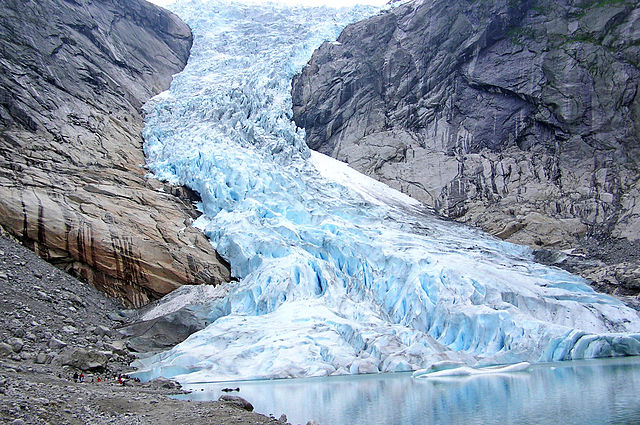
\includegraphics[height=4cm]{Briksdalsbreen.jpg}
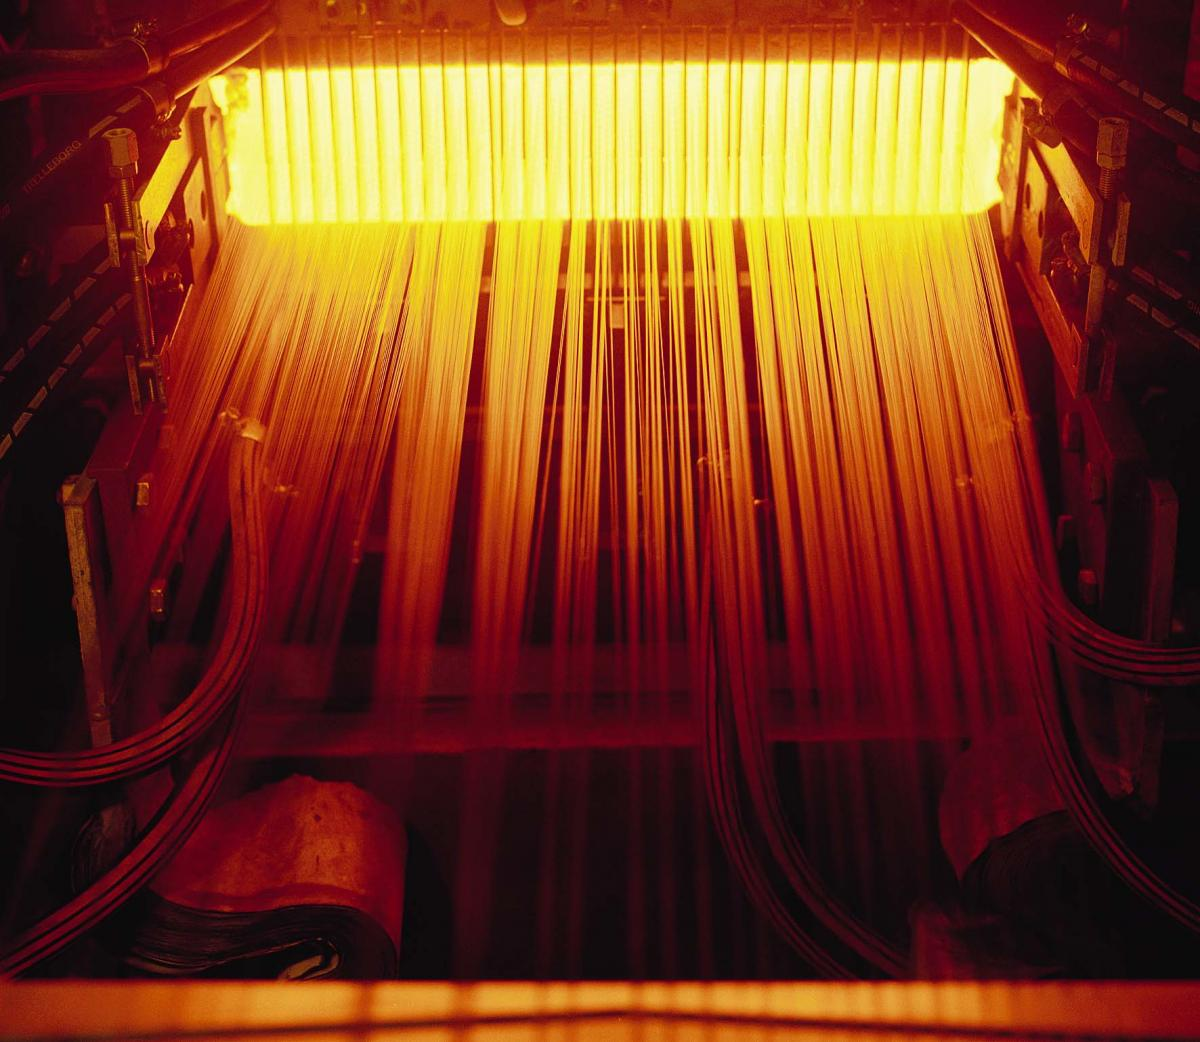
\includegraphics[height=4cm]{fiberglass.jpg}
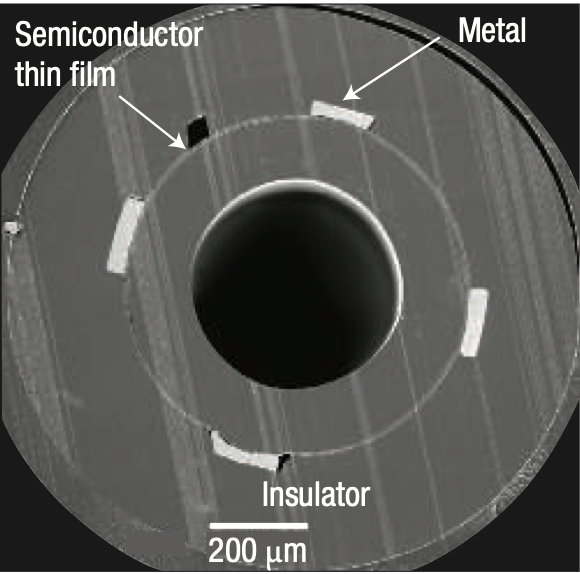
\includegraphics[height=4cm]{sorin.png}
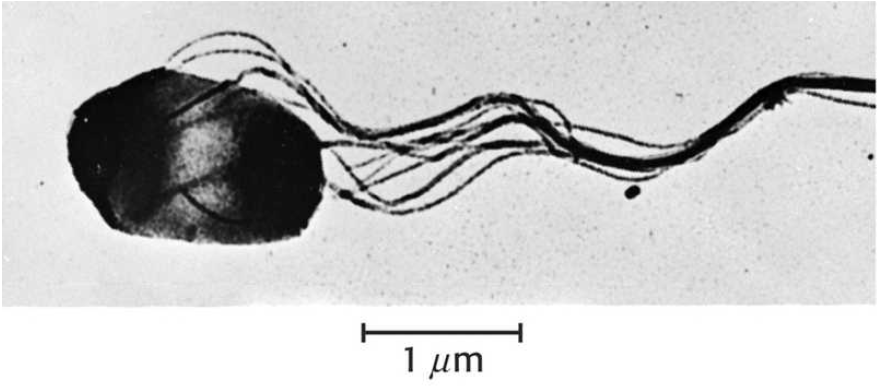
\includegraphics[width=15cm]{salmonella.png}
\caption{\textbf{Flows dominated by viscosity.} Top left : the Briksdalsbreen glacier in Norway is slowly flowing into a lake (photograph by vicrogo, public domain). Top middle: glass fibre manufacturing (photograph Saint-Gobain). Top right: modern optical fibre drawing process allow to produce multilayered fibres \citep{Abouraddy2007}. Bottom: micron-sized salmonellae swim with the help of a bundle of rotating helicoidal flagellae \citep{Elgeti2015}.}
\label{fig:viscous_flows}
\end{center}
\end{figure}

\section{Low-Re number flows}
Whenever fluids have a high viscosity $\mu$, or flow at small scale $L$ or with a low velocity $U$, the equations describing their motion can be greatly simplified. This can be seen by non dimensionalising the equations of motions with the natural scales of the problem $\bU=U\bu$, $\bX=L\bx$ (here we denote dimensioned quantities with capital letters). The pressure can be made dimensionless with a natural viscous scale $P=\mu\frac{U}{L}p$ and finally if there is a imposed timescale $\omega^{-1}$ (e.g. the inverse of the swimming frequency) we may write $T=\omega^{-1}t$.
\begin{equation}
\mathrm{Re}_\omega\pd{\bu}{t} + \mathrm{Re}\lp\bu\cdot\nabla\rp\bu=-\nabla p+\Delta \bu.
\label{eq:pre-stokes_equation}
\end{equation}
Here, two Reynolds numbers appear:
\begin{equation}
\mathrm{Re}_\omega=\frac{\rho L^2 \omega}{\mu} \quad \text{and} \quad \mathrm{Re}=\frac{\rho U L}{\mu},
\end{equation}
which each may be interpreted as a ratio of timescales as seen in the introduction of this chapter. Note that for e.g. flagellae propelled microorganisms, the oscillatory Reynolds number $\mathrm{Re}_\omega$ involves the relevant velocity scale $L\omega$ for the fluid set into motion by the oscillating flagella.

In equation~\eqref{eq:pre-stokes_equation} each variable has been rescaled with its expected range of variation range. Therefore each of the force terms (right hand side) is $\mathcal O(1)$ while the unsteady and convective part of momentum variation (left hand side) are respectively of order $\mathrm{Re}_\omega$ and $\mathrm{Re}$. For flows without an imposed frequency (flowing glass melts or glacier flow), these two numbers will be identical. But if the flow is produced by an oscillating object, they can significantly differ. Table~\ref{tbl:Reynolds} reports an estimation of these two Reynolds numbers for a range of organisms living in aqueous environments, where it can be seen that the double condition $\mathrm{Re}_\omega\ll 1$, $\mathrm{Re}\ll 1$ is fulfilled in the realm of microorganisms.
\begin{table}
\begin{center}
\begin{tabular}{ccccccc}
Organism & length & velocity & frequency & Re & Re$_\omega$\\
\hline\hline
\textbf{Bacterium} & 10 $\mu$m & 10 $\mu$m/s & 100 Hz & \textbf{10$^\text{-4}$} & \textbf{10$^\text{-2}$}\\
\textbf{Spermatozoon} & 100 $\mu$m & 100 $\mu$m/s & 10 Hz & \textbf{10$^\text{-2}$} & \textbf{10$^\text{-1}$}\\
\textbf{Ciliate} & 100 $\mu$m & 1 mm/s & 10 Hz & \textbf{10$^\text{-1}$} & \textbf{10$^\text{-1}$}\\
Tadpole & 1 cm & 10 cm/s & 10 Hz & 10$^\text{3}$ & 10$^\text{3}$\\
Small fish & 10 cm & 10 cm/s & 10 Hz & 10$^\text{4}$ & 10$^\text{5}$\\
Penguin & 1 m & 1 m/s & 1 Hz & 10$^\text{6}$ & 10$^\text{6}$\\
Sperm whale & 10 m & 1 m/s & 0.1 Hz & 10$^\text{7}$ & 10$^\text{7}$\\
\hline
\end{tabular}
\end{center}
\caption{\textbf{Reynolds number for different living organisms.} Bacteria, spermatozoa and ciliates are all characterised by Reynolds numbers Re and Re$_\omega$ much smaller than unity. The flowing fluid in their vicinity is therefore accurately described with the Stokes equation. Data from \citet{Lauga2020}.}
\label{tbl:Reynolds}
\end{table}

In this limit, the Navier-Stokes equation reduces to the much simpler \textbf{Stokes equation}\index{Stokes equation}:
\begin{equation}
\nabla p=\Delta \bu\quad\text{or, in its dimensioned version:}\quad\nabla P=\mu\Delta \bU.
\end{equation}

\prg{Cauchy equation.} Remark that the Stokes equation may also be rewritten as the following \textit{Cauchy equation}:
\begin{equation}
\nabla\cdot\tensorsym\sigma=\matrixsym 0.
\end{equation} 
With this formulation it becomes apparent that viscous flows are \textit{force free}: in absence of significant inertia, the forces balance each other.

\section{The surprising properties of Stokes flows}
Linearity 
Reversibility

\section{Moving in a viscous world}
A paradigm for motion in viscous fluids is the settlement of a sphere, first investigated by Stokes. Arguably lengthy calculations (see tutorial) allow to obtain the expression for the velocity and pressure field around a sphere of radius $R$ settling steadily at velocity $-\bV^\infty$ in a quiescent viscous fluid in its reference frame:
\begin{subequations}
\label{eq:stokes_sphere}
\begin{empheq}[left=\empheqlbrace]{alignat=2}
u_i &\,=\,&& -\frac{3R}{4}V^\infty_j\lp\frac{\delta_{ij}}{r}+\frac{r_ir_j}{r^3}\rp -\frac{3R^3}{4}V^\infty_j\lp\frac{\delta_{ij}}{3r^3}-\frac{r_ir_j}{r^5}\rp,\\
p-p_\infty&\,=\,&&-\frac{3\mu R}{2}\frac{V^\infty_jr_j}{r^3}.
\end{empheq}
\end{subequations}
\begin{figure}[htbp]
\begin{center}
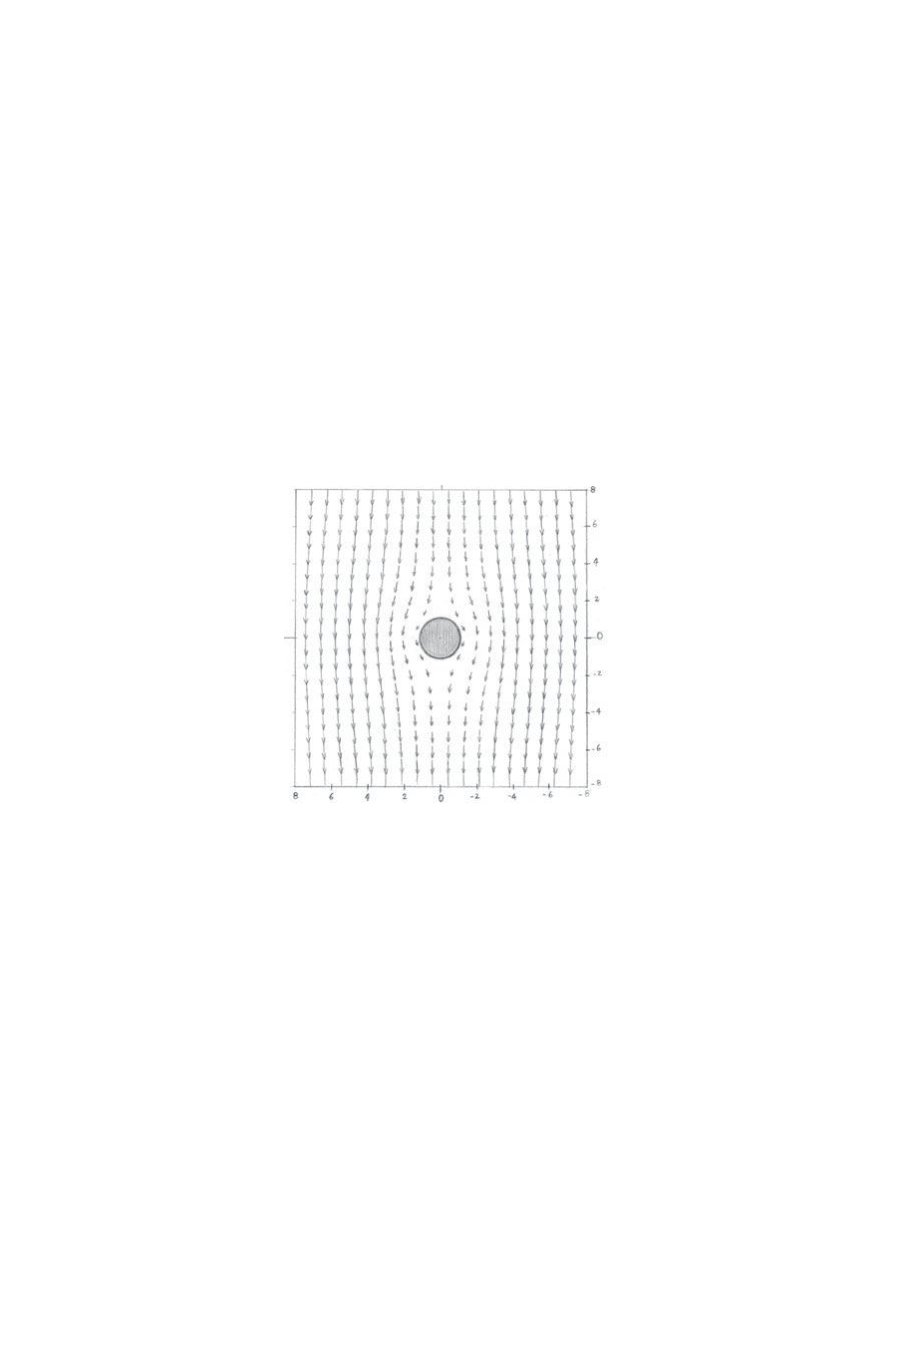
\includegraphics{guazzelli_fixed_sphere.pdf}
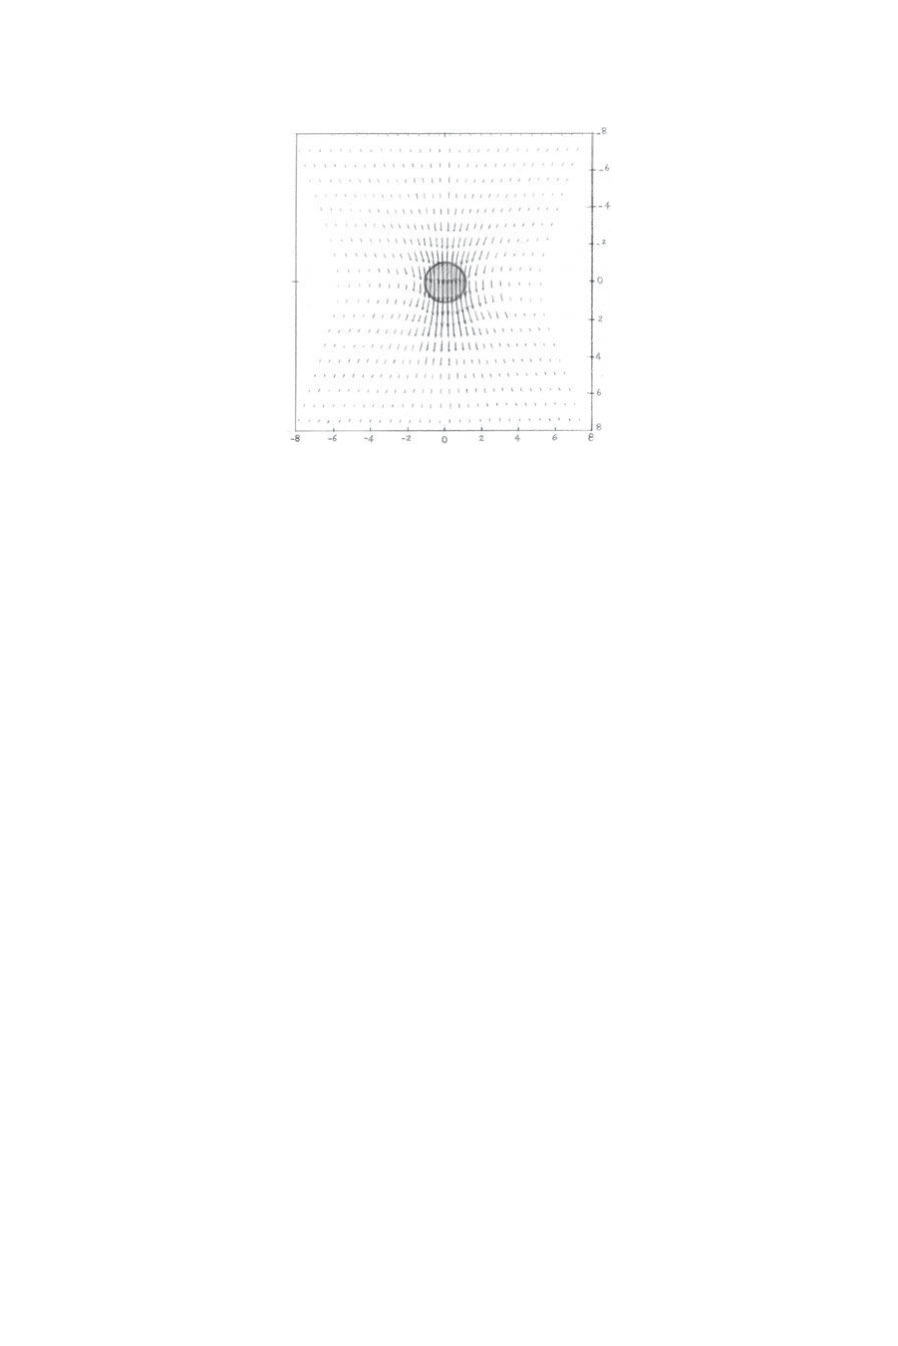
\includegraphics{guazzelli_moving_sphere.pdf}
\caption{\textbf{Spheres in viscous flows}. Left: A fixed sphere deflects the surrounding flowing fluid. Right: A moving sphere in a still environment pushes the fluid in its vicinity \citep{Guazzelli2011}.}
\label{fig:viscous_spheres}
\end{center}
\end{figure}
These expressions allow to evaluate the stresses at the sphere surface and to deduce the well-known \textbf{Stokes drag}\index{Stokes drag}  $\bF = 6 \pi \mu R \bV^\infty$ exerted on the sphere.

An alternative and very useful viewpoint is to present these results in terms of the force $\mathbf f=-\bF$ exerted by the sphere on the fluid:
\begin{equation}
u_i \,=\, \underbrace{\frac{1}{8 \pi\mu R}f_j\lp\frac{\delta_{ij}}{r}+\frac{r_ir_j}{r^3}\rp}_\text{Stokeslet contribution} +\frac{R^2}{8\pi\mu R}f_j\lp\frac{\delta_{ij}}{3r^3}-\frac{r_ir_j}{r^5}\rp.
\end{equation}
Interestingly if we were to shrink the size of the sphere to 0 while keeping the force constant, the only remaining term in the flow field would be the first one. This so-called Stokeslet contribution is of fundamental importance in suspension dynamics, bacteria hydrodynamics and more generally in the modelling of viscous flows.
\subsection{Point force induced flow: the Stokeslet\index{Stokeslet}}
The Stokeslet is a fundamental solution for the Stokes equation, and describes the flow that would be induced by a point force $\mathbf f\, \delta(\bx-\bx_0)$ located at $\bx = \bx_0$. The corresponding velocity and pressure fields therefore satisfy the following \textit{forced Stokes equation}:
\begin{equation}
-\nabla p + \mu \Delta \bu + \mathbf f \,\delta(\bx-\bx_0) = \matrixsym 0.
\label{eq:forced_stokes_equation}
\end{equation}
Note that in this expression $\mathbf f$ is a constant vector. 

The flow field solution is termed \textbf{Stokeslet} and is characterized by: 
\begin{equation}
\left.\bu_{\text{stokeslet}}\right|_i(\bx)=\frac{1}{8\mathrm\pi\mu}\mathcal S_{ij}(\bx |\bx_0) f_j,
\label{eq:stokeslet_velocity_component}
\end{equation}
with $\mathcal S_{ij}$ being the \textit{Oseen-Burgers tensor} defined as:
\begin{equation}
\mathcal S_{ij}=\frac{\delta_{ij}}{r}+\frac{r_i r_j}{r^3}.
\end{equation}
Let's now see in more details how this solution is constructed. To so so it will prove useful to first introduce the Green's function for Laplace equation $g(\bx |\by)$.
\prg{Green's function\index{Green's function} for Laplace equation.} The Green's function $g(x|y)$ for Laplace equation is the function satisfying:
\begin{equation}
\Delta g(\bx |\by) = \delta\lp\bx-\by\rp.
\end{equation}
It is an harmonic function of space except at the point $\bx=\by$ where it is singular. Symmetry considerations on this function suggest that it only depends on the radius $r = \left\|\bx-\by\right\|$. On integrating over a small ball containing the singularity we get:
$$
\oiint \pd{g}{r} \mathrm dS = 1,
$$
so that the Green's function for Laplace equation is:
\begin{equation}
g(\bx |\by) = -\frac{1}{4\mathrm{\pi}r}.
\end{equation}
\prg{Stokeslet obtention.} With the help of the Green's function for Laplace equation, the divergence of the forced Stokes equation~\eqref{eq:forced_stokes_equation} may be written as
\begin{equation}
\Delta\lp p-\mathbf f\cdot\nabla\lp-\frac{1}{4\pi r}\rp\rp = 0.
\end{equation}
The maximum principle for harmonic functions allows us to directly write the pressure as:
\begin{equation}
p=\mathbf f\cdot\nabla\lp-\frac{1}{4\pi r}\rp.
\end{equation}
Injecting this form for the pressure in equation~\eqref{eq:forced_stokes_equation} we obtain:
\begin{equation}
\mu \Delta u_i=\frac{1}{4\mathrm\pi}\lp\underbrace{\delta_{ij}\pd{}{x_k}\pd{}{x_k}}_{\tensorsym I \Delta}\lp\frac{1}{r}\rp-\underbrace{\pd{}{x_i}\pd{}{x_j}}_{\nabla\nabla}\lp\frac{1}{r}\rp\rp f_j.
\label{eq:stokeslet_velocity_laplacian}
\end{equation}
From the structure of this relationship, the adventurous reader might tempt to look for a solution of the form:
\begin{equation}
 u_i=\frac{1}{4\mathrm\pi}\lp\delta_{ij}\Delta \mathcal H-\pd{^2\mathcal H}{x_ix_j}\rp f_j.
\label{eq:stokeslet_velocity_form}
\end{equation}
Note that this velocity field is solenoidal, as:
\begin{equation}
 u_{i,i}=\frac{1}{4\mathrm\pi}\lp\Delta \mathcal H_{,j}-\Delta \mathcal H_{,j}\rp f_j \equiv 0.
\end{equation}
Injecting~\eqref{eq:stokeslet_velocity_form} into~\eqref{eq:stokeslet_velocity_laplacian} we get:
\begin{equation}
\frac{1}{4\mathrm\pi}\lp\tensorsym I\delta-\nabla\nabla\rp\lp\mu\Delta\mathcal H-\lp\frac{1}{r}\rp\rp=0.
\end{equation}
This reduces to the following Poisson equation for $\mathcal H$\footnote{Note that we did not consider the integration constants because they would not appear in the velocity field expression anyway.}:
\begin{equation}
\mu\Delta\mathcal H=\frac{1}{r} \quad\text{with solution:}\quad\mathcal H=\tfrac{1}{2\mu}r.
\end{equation}
Noting that $r=\lp r_kr_k\rp^{1/2}$, we deduce:
\begin{equation}
r_{,i}=\frac{r_{k,i}r_k}{(r_mr_m)^{1/2}}\equiv\frac{x_i}{r} \quad \text{and similarly} \quad r_{,ij}=\frac{\delta_{ij}}{r}-\frac{r_ir_j}{r^3},
\end{equation}
to finally obtain the expression of the Stokeslet velocity field~\eqref{eq:stokeslet_velocity_component} we were looking for:
\begin{equation}
\bu_\text{stokeslet}=\frac{1}{8\pi\mu}\tensorsym S \mathbf f.
\end{equation}
%Superposition
%
%\section{Bacterial hydrodynamics}
%
%Waving sheet Taylor
%
%Scallop theorem
%
%Bacteria with flagellae
%
%\section{Flows at the nanoscale}
%Slip length
